\documentclass[tikz,11pt,border=10pt]{standalone}
%\documentclass[a4paper]{article}

\usepackage{tikz}
\usetikzlibrary{mindmap}

\pgfdeclarelayer{background}
\pgfdeclarelayer{foreground}
\pgfsetlayers{background,main,foreground}

\begin{document}

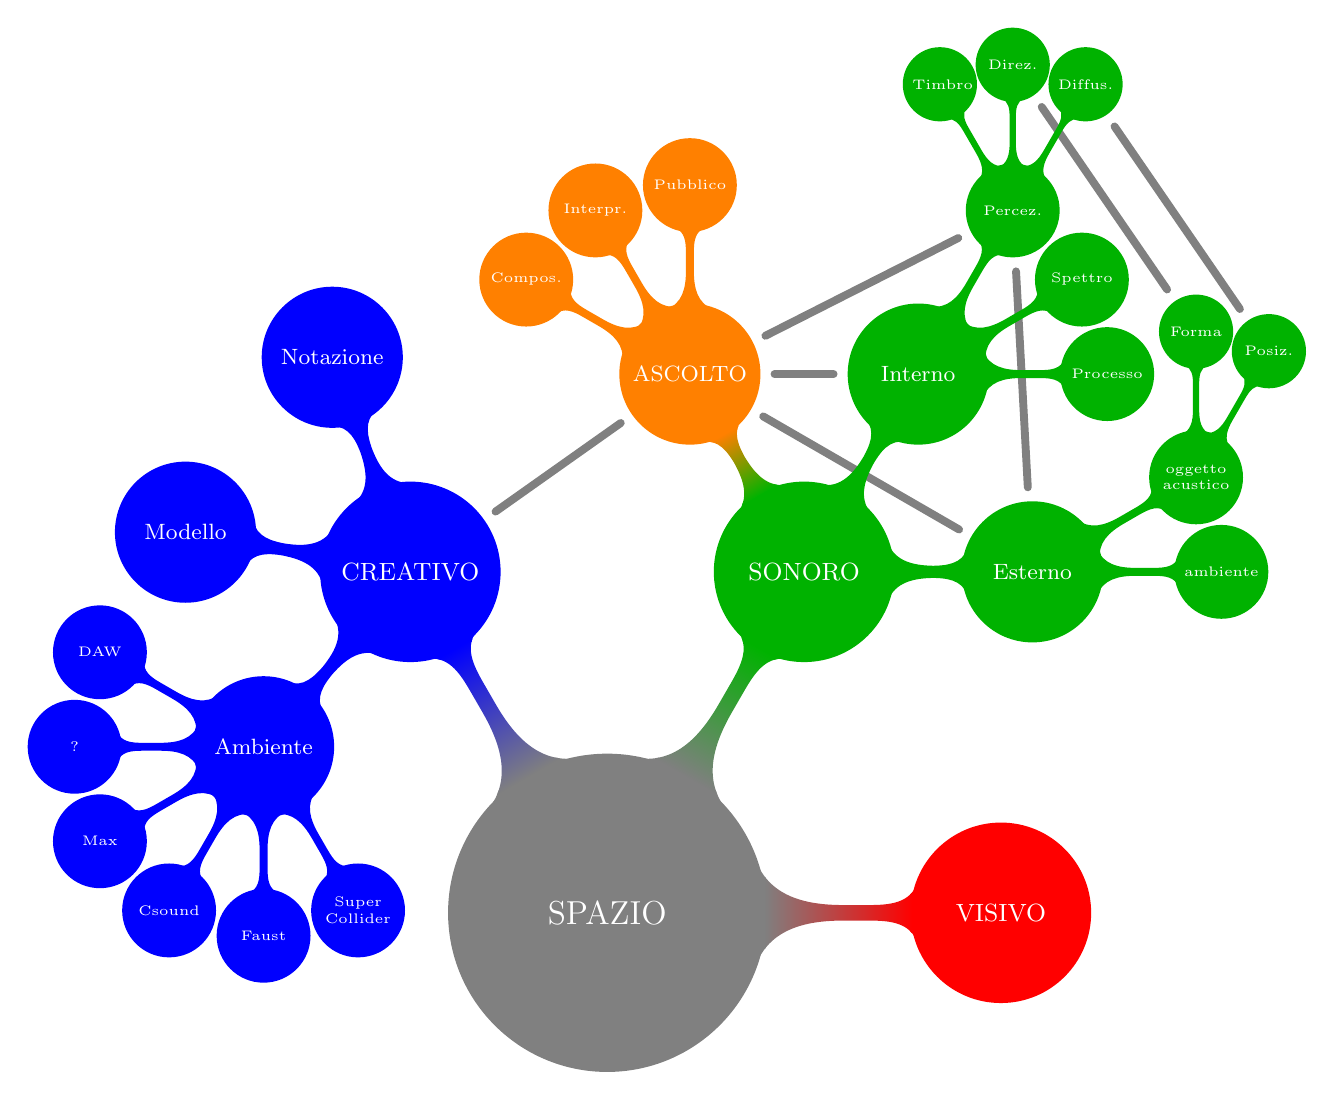
\begin{tikzpicture}
	\path[mindmap,concept color=gray,text=white]
	node[concept] {SPAZIO}
	[clockwise from=120]
		child[concept color=blue] {
		node[concept] (cre) {CREATIVO}
		[clockwise from=230]
	    child {
	    	node[concept] (amb) {Ambiente}
		    [clockwise from=300]
			child {
			node[concept] {Super Collider} }
			child {
				node[concept] {Faust} }
			child {
				node[concept] {Csound} }
			child {
				node[concept] {Max} }	
			child {
				node[concept] {?} }		
			child {
				node[concept] {DAW} }		
		}
		child { node[concept] (aut) {Modello} }	
		child { node[concept] (aut) {Notazione} }				
	}
    child[concept color=green!70!black] {
		node[concept] (son) {SONORO}
		[clockwise from=120]
		child[concept color=orange] {
    		node[concept] (asc) {ASCOLTO}
			[clockwise from=150]
    		child { node[concept] (cmp) {Compos.} }
			child { node[concept] (interp) {Interpr.} }
    		child { node[concept] (pub) {Pubblico} }
		}
		child { node[concept] (int)  {Interno}
			[clockwise from=60]
			child {
				node[concept] (perc) {Percez.}
				[clockwise from=120]
				child { node[concept] (tim) {Timbro } }
				child { node[concept] (dir) {Direz.} }
				child { node[concept] (dif) {Diffus.} }
			}
			child { node[concept] (spet) {Spettro} }
			child { node[concept] (prc) {Processo} }
		}
		child {
			node[concept] (est) {Esterno}
		    [clockwise from=30]
		    child { node [concept] (ogg) {oggetto acustico}
			    [clockwise from=90]
				child { node[concept] (frm) {Forma} }
				child { node[concept] (pos) {Posiz.} }
			}
			child { node [concept] (amb) {ambiente} }			
		}
    }
	child[concept color=red] {
    	node[concept] (vis) {VISIVO}
	};
%	\draw[thick] (node cs:name=son) -- (node cs:name=asc);
%	\draw[thick] (node cs:name=asc) -- (node cs:name=cre);
%	\draw[thick] (node cs:name=est) -- (node cs:name=asc);

\begin{pgfonlayer}{background}
	\draw [concept connection]  (asc) edge (son)
									  edge (cre)									  
									  edge (int)
									  edge (est)
									  edge (perc)
								(est) edge (perc)
								(pos) edge (dif)
								(frm) edge (dir);
\end{pgfonlayer}

\end{tikzpicture}

\end{document}
